\documentclass{article}
\usepackage[utf8]{inputenc}
\usepackage[T2A]{fontenc}
\usepackage[russian]{babel}
\usepackage{graphicx}
\usepackage{amsmath}
\usepackage{amssymb}
\usepackage{bm}
\usepackage[thinc]{esdiff}
\usepackage{mathtools}
\usepackage{breqn}
\usepackage{amsthm}
\usepackage{amsfonts}
\usepackage{bbm}

%Русская традиция
\renewcommand{\leq}{\leqslant}
\renewcommand{\geq}{\geqslant}
\renewcommand{\phi}{\varphi}
\DeclareMathOperator*{\argmax}{argmax}

\theoremstyle{definition}
\newtheorem{definition}{Определение}
\newtheorem*{definition*}{Определение}
\theoremstyle{theorem}
\newtheorem{theorem}{Теорема}
\theoremstyle{remark}
\newtheorem{remark}{Замечание}
\theoremstyle{theorem}
\newtheorem{corollary}{Следствие}
\theoremstyle{example}
\newtheorem{example}{Пример}
\theoremstyle{theorem}
\newtheorem{statement}{Утверждение}
\theoremstyle{theorem}
\newtheorem{alg}{Алгоритм}
\theoremstyle{theorem}
\newtheorem{sug}{Предположение}
\theoremstyle{theorem}
\newtheorem{lemma}{Лемма}

\begin{document}

\tableofcontents

\newpage

\section{ Компоненты свёрточной нейрнной сети}
	\begin{definition}
		Изображение~--- тензор $M\in\mathbb R^{m\times n\times d}$, $m$~--- ширина изображения, $n$~--- длина. Чаще всего $d=3$ (3 канала~--- Red, Green, Blue). 
	\end{definition}
	Учитывая, что обычно рассматривают трёхканальные или четырёхканальные изображения, можно под словом "тензор" понимать трёхмерный или четырёхмерный массив.
	
	Пусть $X \in\mathbb R^{m\times n\times d}$~--- случайная величина "изображение".
	
	Рассматриваются следующие задачи для изображений:
	\begin{itemize}
		\item Классификация $f:X\to\{1,\ldots,K\}$, $K$~--- число классов
		\item Сегментация (1 объект) $f:X\to Y$, $Y\in[0,1]^{m\times n}$, $Y_{ij}=\Prob(X_{ij}\in\text{segment})$, где $\text{segment}$~--- множество точек изображения (пикселей), принадлежащих объекту. Понятно, что можно обобщить на  сегментацию нескольких классов объектов.
	\end{itemize}
	\subsection{Свёртка}
		\begin{definition}
			Пусть $f,g:\mathbb R^n\to\mathbb R$, интегрируемые на $\mathbb R^n$. \textit{Свёрткой} будем называть функцию $f*g:\mathbb R^n\to\mathbb R$, равную $(f*g)(x)=\int\limits_{\mathbb R^n}f(y)g(x-y)dy$
		\end{definition}
		
		Далее под свёрткой будем понимать следующее определение.
		
		\begin{definition}
		Рассмотрим $M\in\mathbb{R}^{m\times n}$~--- изображение по одному из каналов, $K\in\mathbb R^{k\times l}$~--- ядро, \textit{свёрткой изображения относительно отображения $h:\mathbb{R}^{m\times n}\times\mathbb R^{k\times l}\to\mathbb R$ называется функция $*$}, рассмотрим, $(M*K)(i,j)=\sum\limits_{a=1}^k\sum\limits_{b=1}^l M_{i+a,j+b}K_{ab}$. $(M*K)\in\mathbb R^{(m-k+1)\times(n-l+1)}$
	\end{definition}
	
	Для того чтобы размер изображения после свёртки был равен исходному изображению можно как-нибудь заполнить края изображения (padding). Идея аналогична скользящему среднему с синхронизацией в центральной точке. 
	 В основном используются следующие способы padding:
	 \begin{itemize}
	 	\item zeros --- заполнение нулями.
	 	\item reflect --- "отражение", например, вектор $(1,2,3)$ при padding размера 2 отобразится в вектор $(3,2,1,2,3,2,1)$.
	 	\item replicate --- заполнение крайними значениями.
	 	\item circular --- круговое заполнение, вектор $(1,2,3)$ преобразуется в $(2,3,1,2,3,1,2)$.
	 \end{itemize}
	 \begin{figure}[h!]
	 	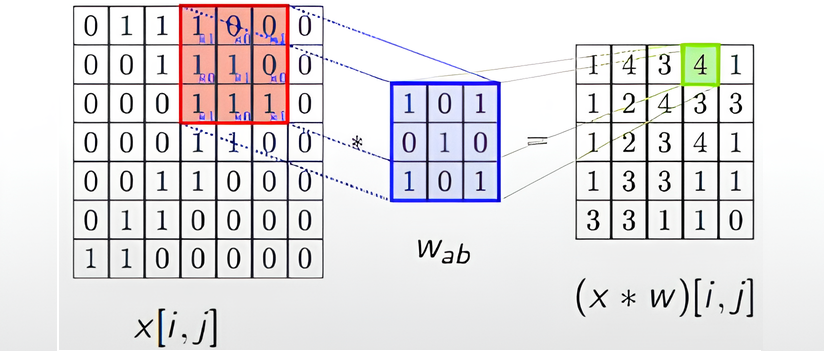
\includegraphics[width=\textwidth]{cnn.png}\caption{Операция свёртки}
	 \end{figure}
	 \newpage
	 \begin{figure}[h!]
	 	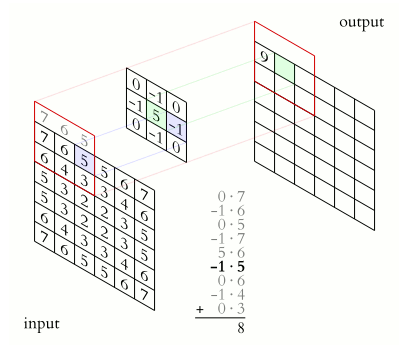
\includegraphics[width=\textwidth]{pollingexample.png}\caption{Операция свёртки}
	 \end{figure}
	 \subsection{Свёрточный слой}
	 	Свёрточный слой задаётся следующими параметрами:
	 	\begin{itemize}
	 		\item Размер ядер $k\times l$ , $k\leq m$, $l\leq n$, $r\in\mathbb N$ число ядер
	 		\item Способ заполнения краёв (padding)
	 		\item Размер заполнения краёв $P\in \mathbb N_0$
	 		\item Величина сдвига ядра (stride) $S\in R^2$. Например, для $S=(1,1)$ получаем операцию, похожую на операцию вложения в 2D-SSA.
	 	\end{itemize}
	 \subsection{ Pooling слой}
	 	Свёрточная нейросеть помимо свёрточных слоёв состоит из pooling слоёв
	 	\begin{definition}
	 		Рассмотрим одноканальное изображение (матрицу)  $M$ размера $m\times n$. Выберем $p$ и $q$, кратные $m$ и $n$ соответственно. Разобьём матрицу на дизъюнктные подматрицы размера $k\times l$ $P_{ij}=\{M_{(i-1)p+k,(j-1)q+l}\}_{k=1,l=1}^{p,q}$, $i\in1:\frac mp$, $j\in1:\frac nq$. \textit{Операция pooling} применяет к каждой матрице $P_{ij}$ некоторую функцию $f$, в результате получается матрица $F$, состоящая из элементов $F(i,j)=f(P_{ij})$.
	 	\end{definition}
	 	
	 	Чаще всего используют max pooling, average pooling и sum pooling.
	 		Pooling слой применяется для уменьшения размерности изображения.
	 	\begin{figure}[ht!]\label{pool}
	 		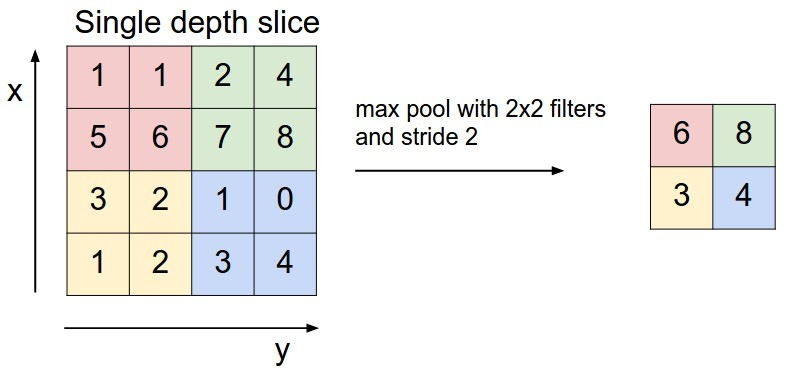
\includegraphics[width=\textwidth]{maxpool.jpeg}\caption{Пример max-pooling}
	 	\end{figure}
	 В случае отсутствия max-pooling слоёв применим алгоритм обратного распространения ошибки. Если присутствуют max-pooling слои, то градиенты пробрасываются в ту клетку, на которой достигается максимум, остальные градиенты равны нулю.
	
	В рис.~\ref{pool} ненулевые градиенты будут в точках $(2,2), (2,4), (3,1), (4,4)$.
	
	На практике не встречается использование min-pooling потому что в случае его использования может произойти затухание градиентов.
	\\В контексте операции подвыборки (pooling), когда говорится о "наличии признака в данных областях", обычно имеется в виду следующее:
	
\textbf{	MaxPooling:}
	
	Если внутри области (например, 2x2 или 3x3) есть какой-либо ярко выраженный признак (например, край объекта, текстура, угол), то максимальное значение в этой области будет высоким.
	MaxPooling выбирает это максимальное значение, предполагая, что оно содержит наиболее важную информацию о наличии этого признака.
	AveragePooling:
	
	Если внутри области есть признаки, но они распределены более равномерно, и нет какого-то одного доминирующего признака, то усредненное значение будет относительно низким.
	\textbf{AveragePooling} усредняет значения, предполагая, что более равномерное распределение признаков может содержать более общую информацию.
	В обоих случаях мы говорим о "признаках" в контексте содержания информации о структуре изображения. Под "признаками" могут пониматься различные аспекты изображения, такие как контуры, текстуры, цвета и т. д. Максимальное или усредненное значение в подвыборке служит метрикой того, насколько выражен или равномерен этот "признак" в данной области.

		
	\section{Свёрточная нейронная сеть}
		В зависимости от постановки задачи после применения свёрточных и pooling слоёв и применения функций активации могут следовать полносвязные или свёрточные  слои. Обычно после применения свёртки следует поэлементное применение функции $\mathrm{ReLU}$, равной $\mathrm{ReLU}(x)=\max(0,x)$ для того, чтобы убрать отрицательные элементы из результатов применения свёрточных слоёв. 
		
		Каждый элемент изображения $M_{ijk}$ показывает интенсивность выбранного пикселя соответствующей координаты и соответствующего канала, в таком случае трудно трактовать отрицательные значения в изображении.
		\newpage
		\begin{figure}[h!]
			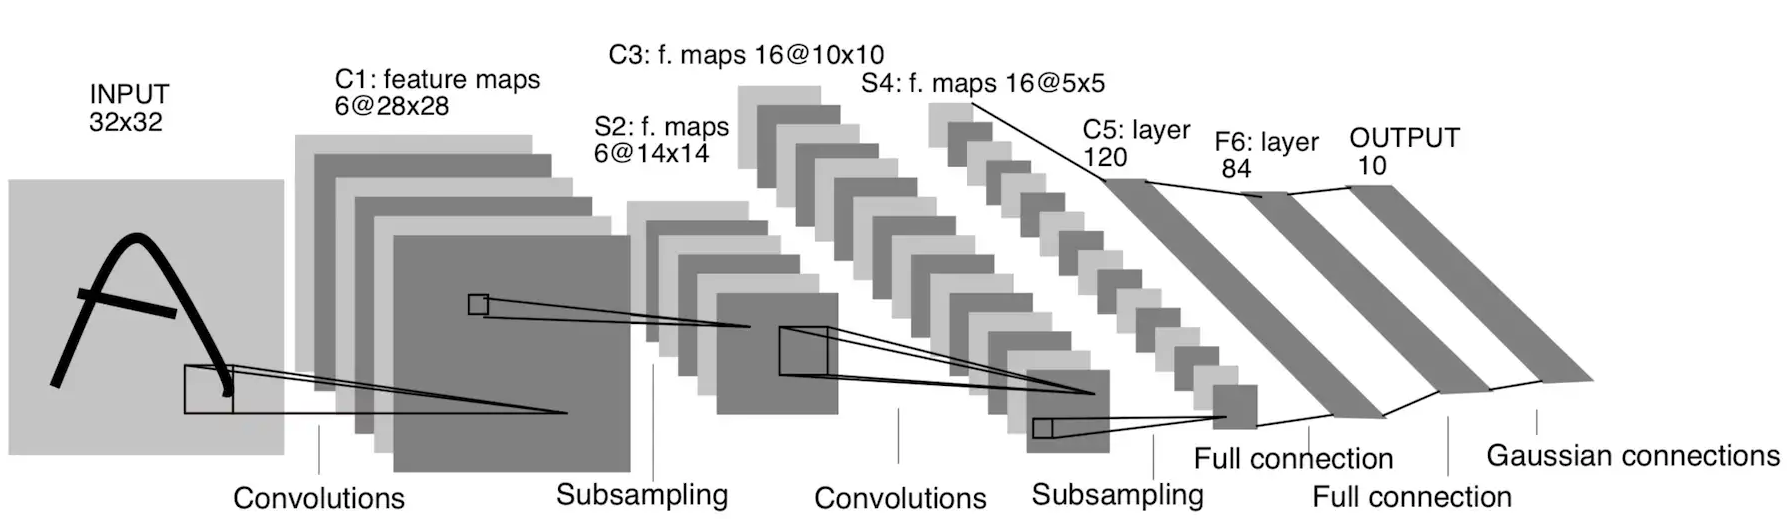
\includegraphics[width=\textwidth]{lesnet.png}\caption{Архитектура сети LeNet}
		\end{figure}
		Рассмотрим пример сети LeNet. На первом шаге применяется 6 свёрток размером $5\times5$, затем max-pooling размером $2\times2$, потом 16 свёрток $5\times 5$  и max-pooling $2\times2$, после этого 16 полученных матриц размером $5\times5$ вытягиваются в один вектор, после которого следует два полносвязанных слоя, и на последнем шаге применяется функция активации $\mathrm{softmax}$. В результате получаем вероятность принадлежности одному из десяти классов для каждого класса.
			\section{Dropout в нейронных сетях}
		
		Dropout — это техника регуляризации, применяемая в нейронных сетях для предотвращения переобучения. Она основана на идее случайного "выключения" (отключения) некоторых нейронов во время обучения.
		
		\subsection{Идея Dropout}
		
		В процессе обучения каждый нейрон в слое с вероятностью $p$ может быть временно отключен (выходить из игры) на текущей итерации обучения. Эта вероятность $p$ называется параметром Dropout. Таким образом, в каждой эпохе обучения структура сети меняется, что помогает предотвратить сильное переобучение.
		
		\subsection{Математическое представление}
		
		Представим, что входной вектор для слоя $l$ — это $\mathbf{x}^{(l)}$, а маска Dropout для этого слоя — это $\mathbf{m}^{(l)}$, где каждый элемент маски является случайной переменной, принимающей значения 0 или 1 с вероятностью $p$. Тогда выход слоя с применением Dropout можно записать следующим образом:
		
		\[
		\mathbf{y}^{(l)} = \mathbf{m}^{(l)} \odot \mathbf{x}^{(l)}
		\]
		
		где $\odot$ — поэлементное умножение (применение маски).
		
		\subsection{Обучение с Dropout}
		
		Во время обучения происходит вычисление градиентов и обновление весов, как обычно. В процессе прямого прохода Dropout применяется, а в процессе обратного прохода градиенты распространяются только через активные (не выключенные) нейроны.
		\begin{figure}[h!]
			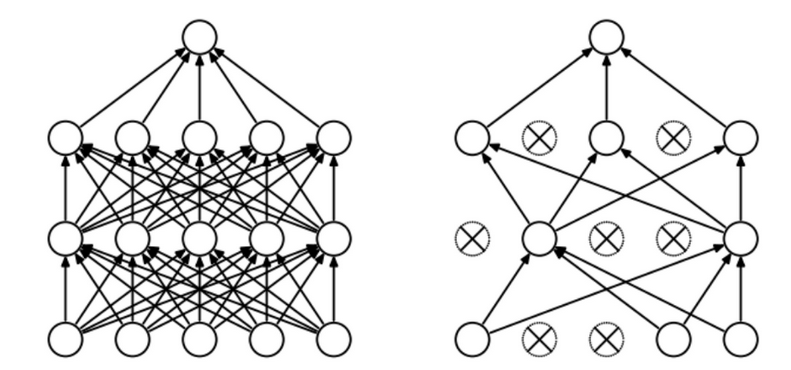
\includegraphics[width=\textwidth]{drop.png}\caption{dropout}
		\end{figure}
		\section{Улчшения качества свёрточных нейросетей} 
			\subsection{Аугументация}
				Одной из проблем работы с изображениями является малое количество размеченных изображений. Обычно изображения размечаются вручную. Для размножения данных используются аугументации.
				
		\begin{definition}
			Аугументация (Augumentation)~--- увеличение объёма тренировочной выборки с помощью различных афинных преобразований изображений: зеркальное отражение, поворот, сдвиг, изменение масштаба.
		\end{definition}
		
		Также аугументации позволяют улучшить качество предсказания на тестовой выборки. Например, наша задача --- определение дорожных знаков по фотографии. Обучающая выборка состоит из дорожных знаков из справочника (сфотографированы "анфас"). Если обучить модель на выборке без аугументаций, то при рассмотрении реальной фотографии дорожных знаков модель может давать плохие результаты потому что как правило встречаются фотографии с некоторыми дефектами в сравнении с изображениями из обучающей выборки: повороты, размытия, сдвиги. Если рассмотреть аугументированную выборке, то в ней будет больше изображений, похожих на реальные и новая модель сможет предсказывать с большей точностью чем модель, обученная на выборке без аугументаций.
		\newpage 
		\begin{figure}[h!]
			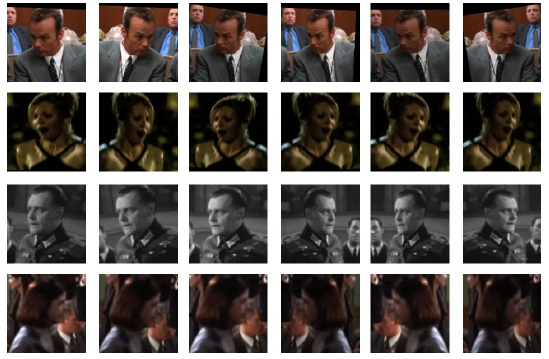
\includegraphics[width=\textwidth]{aug.png}\caption{Пример аугументации изображений}
		\end{figure}
		\section{Применение CNN в обработке аудиофайлов}
		
		\subsection{Спектрограммы и свертка}
		
		CNN могут эффективно использоваться для анализа аудиосигналов в виде спектрограмм. Спектрограмма представляет собой изображение, отражающее изменения частоты во времени. Сверточные слои в сети могут обнаруживать различные звуковые паттерны и особенности в разных участках времени.\\
		
		\begin{figure}[h!]
			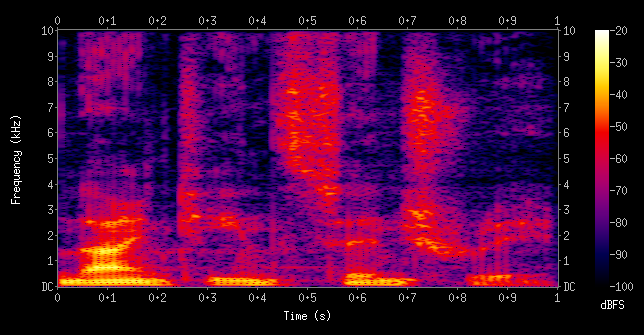
\includegraphics[width=\textwidth]{spec.png}\caption{Спектрограмма}
		\end{figure}
		
		\subsection{Обработка последовательности звуковых данных}
		
		Сверточные нейронные сети могут быть применены для обработки временных последовательностей звуковых данных. В этом случае, сверточные слои могут извлекать локальные признаки, такие как изменения громкости или наличие определенных звуковых шаблонов.
		
		\subsection{Использование пулинга для извлечения признаков}
		
		Слой пулинга может использоваться для уменьшения размерности данных, что позволяет сети сосредотачиваться на более важных аспектах звуковой информации. Например, максимальный пулинг может выделять наиболее значимые частотные компоненты в каждом временном интервале.
		
		\subsection{Задачи обработки аудиосигналов с использованием CNN}
		
		CNN могут быть применены для решения различных задач обработки аудиосигналов, таких как:
		\begin{itemize}
			\item Распознавание речи.
			\item Классификация звуковых событий.
			\item Идентификация музыкальных инструментов.
			\item Разделение звуковых дорожек.
		\end{itemize}
	\section{Использование CNN в NLP}
	Последовательные слова в тексте представляются векторами с
	помощью векторных представлений(fastText, word2vec, One-hot
	encoding и тд.)
	\begin{itemize}

	\item \textbf{Классификация текста}
	
	CNN могут быть успешно применены для задачи бинарной или многоклассовой классификации текста. Сверточные слои выступают в роли фильтров, выделяя локальные паттерны в предложениях или текстах.
	
	\item \textbf{Анализ тональности}
	
	В решении задачи определения тональности текста, CNN извлекают контекстуальные признаки из последовательности слов, позволяя выявлять позитивные, негативные или нейтральные настроения.
	
	\item \textbf{Извлечение признаков из текста}
	
	Сверточные слои могут быть использованы для извлечения важных признаков из текстовых данных. Это полезно для создания эмбеддингов, представляющих слова или фразы в векторной форме.
	
	\item \textbf{Детекция именованных сущностей (NER)}
	
	Для задачи NER, CNN применяются для обнаружения и классификации именованных сущностей в тексте.
	
	\item \textbf{Анализ последовательности}
	
	В сочетании с рекуррентными слоями, такими как LSTM или GRU, CNN могут быть использованы для анализа последовательности слов, учитывая контекст в тексте.
	
	\item \textbf{Создание архитектур для задачи NLP}
	CNN могут составлять часть более сложных архитектур, например, TextCNN, которые включают несколько слоев свертки, слоев пулинга и полносвязанных слоев для решения конкретных задач NLP.
	\begin{figure}[h!]
		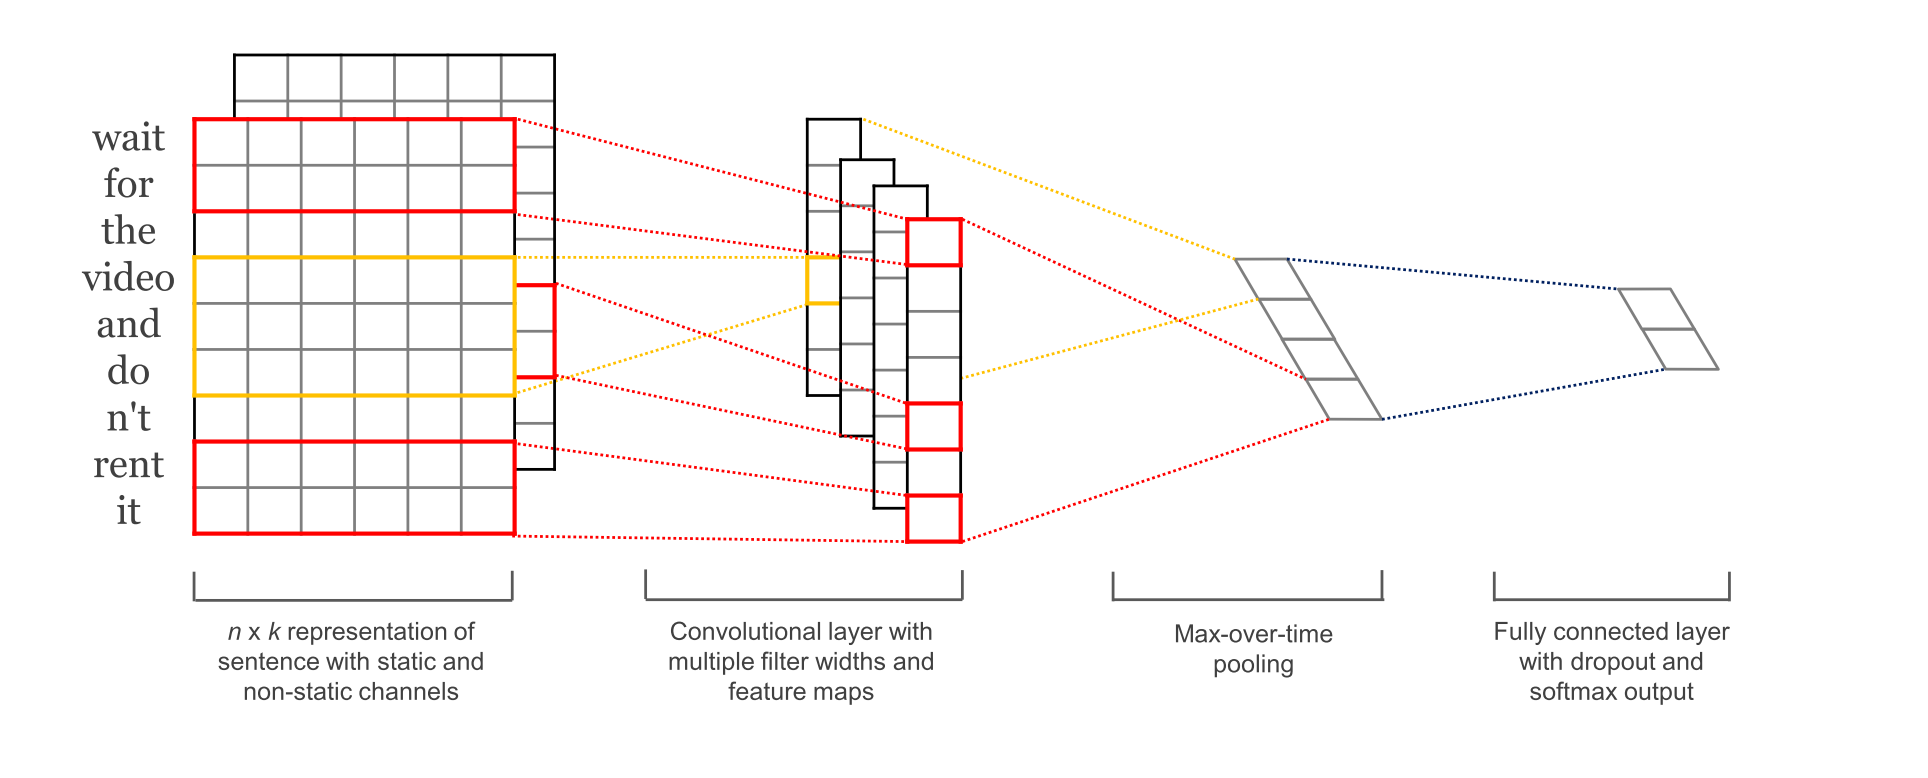
\includegraphics[width=\textwidth]{nlp.png}\caption{Разложение слов на векторы и их дальнейшее преобразования}
	\end{figure}
	\end{itemize}
	\section{ImageNet}
	
	ImageNet — это крупнейшая база данных изображений, используемая в задачах компьютерного зрения и обучения глубоких нейронных сетей. Она играет ключевую роль в развитии и оценке различных архитектур нейронных сетей.
	
	\subsection{Описание}
	
	\begin{itemize}
		\item \textbf{Размер базы данных:} ImageNet содержит более 14 миллионов изображений, представляющих более 20 000 категорий объектов.
		
		\item \textbf{Категории:} Каждое изображение в ImageNet привязано к одной из тысяч категорий, включающих широкий спектр объектов, таких как животные, растения, транспортные средства, еда и многое другое.
		
		\item \textbf{Задачи:} ImageNet используется для нескольких задач, включая классификацию изображений (присвоение каждому изображению одной из категорий), детекцию объектов (обнаружение и классификация объектов на изображении) и локализацию объектов (определение местоположения объектов на изображении).
		
		\item \textbf{Использование в соревнованиях:} ImageNet служит основой для проведения ежегодного соревнования ILSVRC (ImageNet Large Scale Visual Recognition Challenge), в котором исследователи и инженеры создают и сравнивают различные модели глубокого обучения на задачах классификации изображений.
	\end{itemize}
	
	\subsection{Важность для глубокого обучения}
	
	ImageNet стал своего рода эталоном для оценки производительности и обобщающей способности моделей глубокого обучения. Разработка и сравнение моделей на базе данных ImageNet позволяет измерять и сравнивать способность моделей распознавать и классифицировать разнообразные объекты в реальном мире.
	
	
	\section{Выводы}
		Проблемы:
		\begin{itemize}
			\item Необходимость разметки данных для обучения
			\item Большое количество параметром, следовательно долгое обучение, даже на GPU
		\end{itemize}
	Решения:
		\begin{itemize}
			\item Использование размеченных библиотек изображений: ImageNet (14M изображений, 1000 категорий), OpenImages (9М изображений, 60К меток, 20К категория)
			\item Использование модели, обученной на размеченной библиотеке изображений известной архитектуры, например Alexnet, vgg net, Resnet. 
			
		Обычно новые архитектуры публикуются в результате достижения рекордной точности на каком-нибудь соревновании. Например, архитектура vgg 16 показала точность 0.927 на датасете ImageNet на соревновании ImageNet Large Scale Visual Recognition Challenge 2014 и после была опубликована.
		\end{itemize}
		\begin{figure}[h!]
			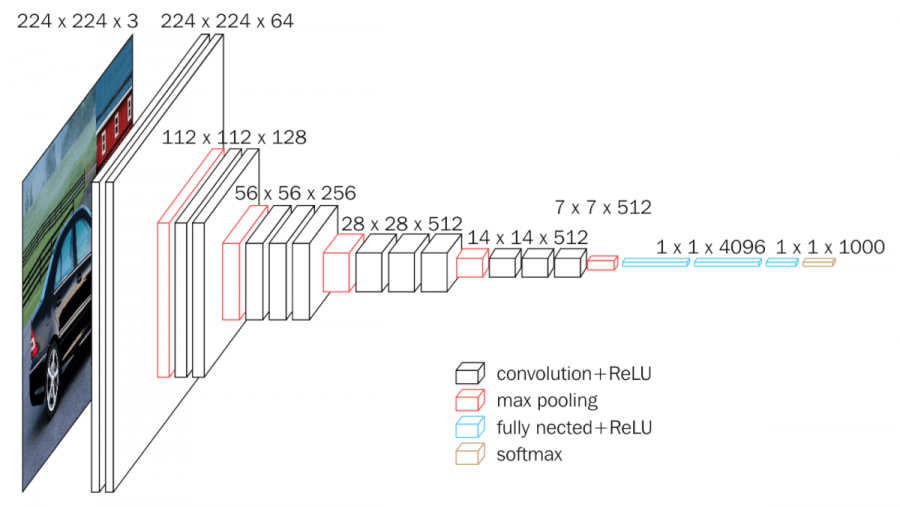
\includegraphics[width=\textwidth]{vgg16.png}\caption{Архитектура сети vgg 16}
		\end{figure}
		\begin{figure}[h!]
			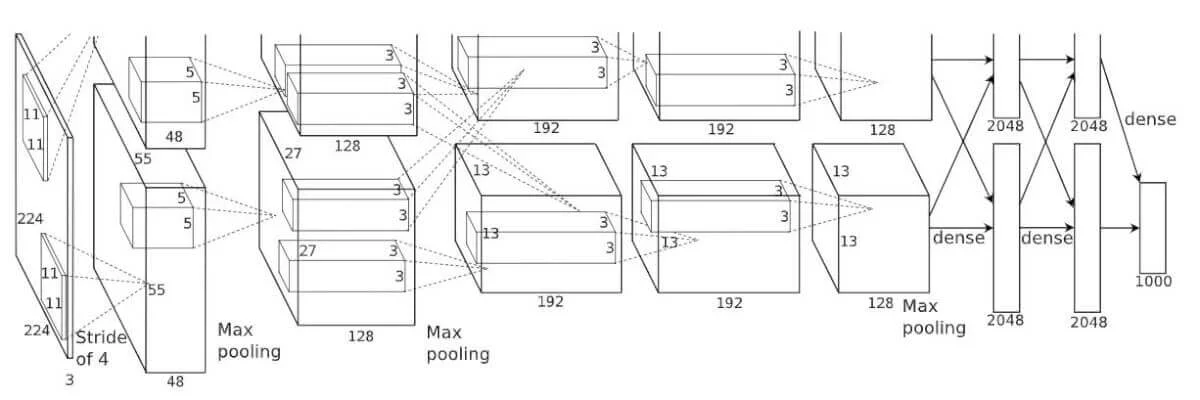
\includegraphics[width=\textwidth]{AlexNet.png}\caption{Архитектура сети AlexNet}
		\end{figure}
		Все эти сети имеют разные(или почти разные конфигурации), но могут быть загружены и использованы для своих нужд. В таком случае, обычно вся архитектура сети загружается со своими полученными весами. Необходимо добавить последний полносвязнный слой, и обучить на ваших данных

\end{document}
